\chapter{Diccionarios}

Este capítulo presenta otro tipo incorporado llamado diccionario. Los diccionarios son una de las mejores características de Python; son los bloques de construcción de muchos algoritmos eficientes y elegantes.

\section{Un diccionario es un mapeo}

Un \textbf{diccionario} es como una lista, pero más general. En una lista, los índices deben ser enteros; en un diccionario pueden ser (casi) cualquier tipo.

Un diccionario contiene una colección de índices, llamados \textbf{claves}, y una colección de valores. Cada clave está asociada a un único valor. La asociación de una clave y un valor se llama \textbf{par clave-valor} o, a veces, un \textbf{ítem}.

En lenguaje matemático, un diccionario representa un \textbf{mapeo} de claves a valores, por lo que también puedes decir que cada clave "mapea a" un valor. Como ejemplo, construiremos un diccionario que mapea palabras del inglés al español, por lo que las claves y los valores son todas cadenas.

La función \texttt{dict} crea un nuevo diccionario sin ítems. Como \texttt{dict} es el nombre de una función incorporada, debes evitar usarlo como nombre de variable.

\begin{lstlisting}[language=Python]
>>> eng2sp = dict()
>>> eng2sp
{}
\end{lstlisting}

Las llaves, \texttt{\{\}}, representan un diccionario vacío. Para agregar ítems al diccionario, puedes usar corchetes:

\begin{lstlisting}[language=Python]
>>> eng2sp['one'] = 'uno'
\end{lstlisting}

Esta línea crea un ítem que mapea la clave \texttt{'one'} al valor \texttt{'uno'}. Si imprimimos el diccionario nuevamente, vemos un par clave-valor con dos puntos entre la clave y el valor:

\begin{lstlisting}[language=Python]
>>> eng2sp
{'one': 'uno'}
\end{lstlisting}

Este formato de salida también es un formato de entrada. Por ejemplo, puedes crear un nuevo diccionario con tres ítems:

\begin{lstlisting}[language=Python]
>>> eng2sp = {'one': 'uno', 'two': 'dos', 'three': 'tres'}
\end{lstlisting}

Pero si imprimes \texttt{eng2sp}, podrías sorprenderte:

\begin{lstlisting}[language=Python]
>>> eng2sp
{'one': 'uno', 'three': 'tres', 'two': 'dos'}
\end{lstlisting}

El orden de los pares clave-valor podría no ser el mismo. Si escribes el mismo ejemplo en tu computadora, podrías obtener un resultado diferente. En general, el orden de los ítems en un diccionario es impredecible.

Pero eso no es un problema porque los elementos de un diccionario nunca se indexan con índices enteros. En su lugar, usas las claves para buscar los valores correspondientes:

\begin{lstlisting}[language=Python]
>>> eng2sp['two']
'dos'
\end{lstlisting}

La clave \texttt{'two'} siempre mapea al valor \texttt{'dos'}, por lo que el orden de los ítems no importa.

Si la clave no está en el diccionario, obtienes una excepción:

\begin{lstlisting}[language=Python]
>>> eng2sp['four']
KeyError: 'four'
\end{lstlisting}

La función \texttt{len} funciona con diccionarios; devuelve el número de pares clave-valor:

\begin{lstlisting}[language=Python]
>>> len(eng2sp)
3
\end{lstlisting}

El operador \texttt{in} también funciona con diccionarios; te dice si algo aparece como clave en el diccionario (aparecer como valor no es suficiente):

\begin{lstlisting}[language=Python]
>>> 'one' in eng2sp
True
>>> 'uno' in eng2sp
False
\end{lstlisting}

Para ver si algo aparece como valor en un diccionario, puedes usar el método \texttt{values}, que devuelve una colección de valores, y luego usar el operador \texttt{in}:

\begin{lstlisting}[language=Python]
>>> vals = eng2sp.values()
>>> 'uno' in vals
True
\end{lstlisting}

El operador \texttt{in} usa diferentes algoritmos para listas y diccionarios. Para listas, busca los elementos de la lista en orden, como en la Sección 8.6. A medida que la lista se alarga, el tiempo de búsqueda aumenta en proporción directa.

Los diccionarios de Python usan una estructura de datos llamada \textbf{tabla hash} que tiene una propiedad notable: el operador \texttt{in} toma aproximadamente la misma cantidad de tiempo sin importar cuántos ítems haya en el diccionario. Explicaré cómo es posible esto en la Sección B.4, pero la explicación podría no tener sentido hasta que hayas leído algunos capítulos más.

\section{Diccionario como una colección de contadores}

Supongamos que te dan una cadena y quieres contar cuántas veces aparece cada letra. Hay varias formas de hacerlo:

\begin{enumerate}
    \item Podrías crear 26 variables, una para cada letra del alfabeto. Luego podrías recorrer la cadena y, para cada carácter, incrementar el contador correspondiente, probablemente usando un condicional encadenado.
    \item Podrías crear una lista con 26 elementos. Luego podrías convertir cada carácter a un número (usando la función incorporada \texttt{ord}), usar el número como índice en la lista e incrementar el contador apropiado.
    \item Podrías crear un diccionario con caracteres como claves y contadores como los valores correspondientes. La primera vez que veas un carácter, agregarías un ítem al diccionario. Después, incrementarías el valor de un ítem existente.
\end{enumerate}

Cada una de estas opciones realiza el mismo cálculo, pero cada una implementa ese cálculo de manera diferente.

Una \textbf{implementación} es una forma de realizar un cálculo; algunas implementaciones son mejores que otras. Por ejemplo, una ventaja de la implementación con diccionarios es que no tenemos que saber de antemano qué letras aparecen en la cadena y solo tenemos que hacer espacio para las letras que sí aparecen.

Aquí está cómo podría verse el código:

\begin{lstlisting}[language=Python]
def histogram(s):
    d = dict()
    for c in s:
        if c not in d:
            d[c] = 1
        else:
            d[c] += 1
    return d
\end{lstlisting}

El nombre de la función es \texttt{histogram}, que es un término estadístico para una colección de contadores (o frecuencias).

La primera línea de la función crea un diccionario vacío. El bucle \texttt{for} recorre la cadena. Cada vez que pasa por el bucle, si el carácter \texttt{c} no está en el diccionario, creamos un nuevo ítem con la clave \texttt{c} y el valor inicial 1 (ya que hemos visto esta letra una vez). Si \texttt{c} ya está en el diccionario, incrementamos \texttt{d[c]}.

Así es como funciona:

\begin{lstlisting}[language=Python]
>>> h = histogram('brontosaurus')
>>> h
{'a': 1, 'b': 1, 'o': 2, 'n': 1, 's': 2, 'r': 2, 'u': 2, 't': 1}
\end{lstlisting}

El histograma indica que las letras \texttt{'a'} y \texttt{'b'} aparecen una vez; \texttt{'o'} aparece dos veces, y así sucesivamente.

Los diccionarios tienen un método llamado \texttt{get} que toma una clave y un valor predeterminado. Si la clave aparece en el diccionario, \texttt{get} devuelve el valor correspondiente; de lo contrario, devuelve el valor predeterminado. Por ejemplo:

\begin{lstlisting}[language=Python]
>>> h = histogram('a')
>>> h
{'a': 1}
>>> h.get('a', 0)
1
>>> h.get('c', 0)
0
\end{lstlisting}

Como ejercicio, usa \texttt{get} para escribir \texttt{histogram} de manera más concisa. Deberías poder eliminar la sentencia \texttt{if}.

\section{Bucles y diccionarios}

Si usas un diccionario en una sentencia \texttt{for}, recorre las claves del diccionario. Por ejemplo, \texttt{print\_hist} imprime cada clave y el valor correspondiente:

\begin{lstlisting}[language=Python]
def print_hist(h):
    for c in h:
        print(c, h[c])
\end{lstlisting}

Así es como se ve la salida:

\begin{lstlisting}[language=Python]
>>> h = histogram('parrot')
>>> print_hist(h)
a 1
p 1
r 2
t 1
o 1
\end{lstlisting}

Nuevamente, las claves no están en un orden particular. Para recorrer las claves en orden ordenado, puedes usar la función incorporada \texttt{sorted}:

\begin{lstlisting}[language=Python]
>>> for key in sorted(h):
...     print(key, h[key])
a 1
o 1
p 1
r 2
t 1
\end{lstlisting}

\section{Búsqueda inversa}

Dado un diccionario \texttt{d} y una clave \texttt{k}, es fácil encontrar el valor correspondiente \texttt{v = d[k]}. Esta operación se llama \textbf{búsqueda}.

Pero, ¿qué pasa si tienes \texttt{v} y quieres encontrar \texttt{k}? Tienes dos problemas: primero, podría haber más de una clave que mapee al valor \texttt{v}. Dependiendo de la aplicación, podrías elegir una o tener que hacer una lista que las contenga a todas. Segundo, no hay una sintaxis simple para hacer una búsqueda inversa; tienes que buscar.

Aquí hay una función que toma un valor y devuelve la primera clave que mapea a ese valor:

\begin{lstlisting}[language=Python]
def reverse_lookup(d, v):
    for k in d:
        if d[k] == v:
            return k
    raise LookupError()
\end{lstlisting}

Esta función es otro ejemplo del patrón de búsqueda, pero usa una característica que no hemos visto antes, \texttt{raise}. La sentencia \texttt{raise} provoca una excepción; en este caso, provoca un \texttt{LookupError}, que es una excepción incorporada que se usa para indicar que una operación de búsqueda falló.

Si llegamos al final del bucle, significa que \texttt{v} no aparece en el diccionario como valor, por lo que generamos una excepción.

Aquí hay un ejemplo de una búsqueda inversa exitosa:

\begin{lstlisting}[language=Python]
>>> h = histogram('parrot')
>>> key = reverse_lookup(h, 2)
>>> key
'r'
\end{lstlisting}

Y una no exitosa:

\begin{lstlisting}[language=Python]
>>> key = reverse_lookup(h, 3)
Traceback (most recent call last):
    File "<stdin>", line 1, in <module>
    File "<stdin>", line 5, in reverse_lookup
LookupError
\end{lstlisting}

El efecto cuando generas una excepción es el mismo que cuando Python genera una: imprime un rastreo y un mensaje de error.

Cuando generas una excepción, puedes proporcionar un mensaje de error detallado como argumento opcional. Por ejemplo:

\begin{lstlisting}[language=Python]
>>> raise LookupError('value does not appear in the dictionary')
Traceback (most recent call last):
    File "<stdin>", line 1, in ?
LookupError: value does not appear in the dictionary
\end{lstlisting}

Una búsqueda inversa es mucho más lenta que una búsqueda directa; si tienes que hacerla a menudo, o si el diccionario crece, el rendimiento de tu programa se verá afectado.

\section{Diccionarios y listas}

Las listas pueden aparecer como valores en un diccionario. Por ejemplo, si te dan un diccionario que mapea letras a frecuencias, podrías querer invertirlo; es decir, crear un diccionario que mapee frecuencias a letras. Como podría haber varias letras con la misma frecuencia, cada valor en el diccionario invertido debería ser una lista de letras.

Aquí hay una función que invierte un diccionario:

\begin{lstlisting}[language=Python]
def invert_dict(d):
    inverse = dict()
    for key in d:
        val = d[key]
        if val not in inverse:
            inverse[val] = [key]
        else:
            inverse[val].append(key)
    return inverse
\end{lstlisting}

\begin{figure}[h]
\centering
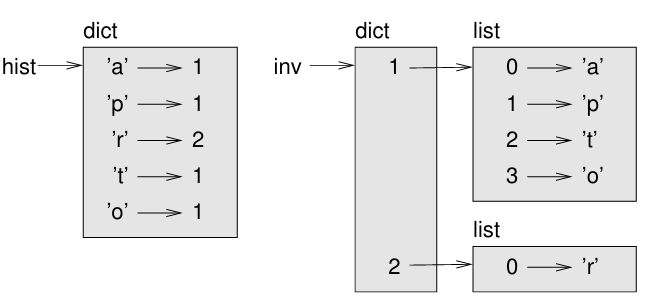
\includegraphics[width=0.7\linewidth]{images/chapter_11_1.png} % Ajusta el nombre del archivo
\caption{Diagrama de estado.}
\label{fig:diagrama_estado}
\end{figure}

Cada vez que pasa por el bucle, \texttt{key} obtiene una clave de \texttt{d} y \texttt{val} obtiene el valor correspondiente. Si \texttt{val} no está en \texttt{inverse}, significa que no lo hemos visto antes, por lo que creamos un nuevo ítem y lo inicializamos con un \textbf{singleton} (una lista que contiene un solo elemento). De lo contrario, hemos visto este valor antes, por lo que agregamos la clave correspondiente a la lista.

Aquí hay un ejemplo:

\begin{lstlisting}[language=Python]
>>> hist = histogram('parrot')
>>> hist
{'a': 1, 'p': 1, 'r': 2, 't': 1, 'o': 1}
>>> inverse = invert_dict(hist)
>>> inverse
{1: ['a', 'p', 't', 'o'], 2: ['r']}
\end{lstlisting}

Las listas pueden ser valores en un diccionario, como muestra este ejemplo, pero no pueden ser claves. Esto es lo que sucede si lo intentas:

\begin{lstlisting}[language=Python]
>>> t = [1, 2, 3]
>>> d = dict()
>>> d[t] = 'oops'
Traceback (most recent call last):
    File "<stdin>", line 1, in ?
TypeError: list objects are unhashable
\end{lstlisting}

Como mencioné antes, un diccionario se implementa usando una tabla hash, y eso significa que las claves deben ser \textbf{hashables}.

Un \textbf{hash} es una función que toma un valor (de cualquier tipo) y devuelve un entero. Los diccionarios usan estos enteros, llamados valores hash, para almacenar y buscar pares clave-valor.

Este sistema funciona bien si las claves son inmutables. Pero si las claves son mutables, como las listas, suceden cosas malas. Por ejemplo, cuando creas un par clave-valor, Python aplica el hash a la clave y la almacena en la ubicación correspondiente. Si modificas la clave y luego aplicas el hash nuevamente, iría a una ubicación diferente. En ese caso, podrías tener dos entradas para la misma clave, o podrías no poder encontrar una clave. De cualquier manera, el diccionario no funcionaría correctamente.

Por eso las claves deben ser hashables, y por qué tipos mutables como las listas no lo son. La forma más sencilla de evitar esta limitación es usar tuplas, que veremos en el próximo capítulo.

\begin{figure}[h]
\centering
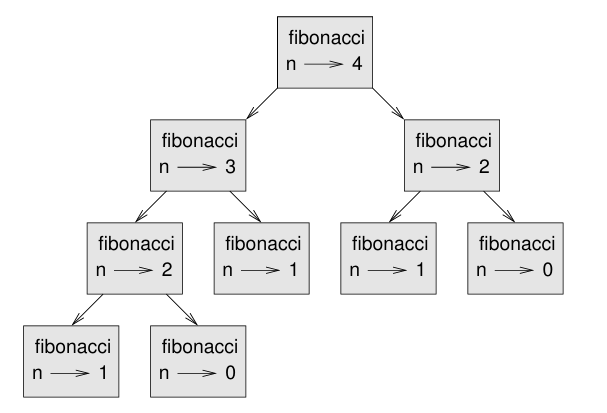
\includegraphics[width=0.7\linewidth]{images/chapter_11_2.png} % Ajusta el nombre del archivo
\caption{Gráfico de llamada.}
\label{fig:diagrama_estado}
\end{figure}

Dado que los diccionarios son mutables, no s epueden usar como claves, pero se pueden usar como valores.

\section{Memorización}

Si jugaste con la función \texttt{fibonacci} de la Sección 6.7, quizás hayas notado que cuanto más grande es el argumento que proporcionas, más tiempo tarda la función en ejecutarse. Además, el tiempo de ejecución aumenta rápidamente.

Para entender por qué, considera la Figura 11.2, que muestra el \textbf{gráfico de llamadas} para \texttt{fibonacci} con \texttt{n=4}:

Un gráfico de llamadas muestra un conjunto de marcos de función, con líneas que conectan cada marco con los marcos de las funciones que llama. En la parte superior del gráfico, \texttt{fibonacci} con \texttt{n=4} llama a \texttt{fibonacci} con \texttt{n=3} y \texttt{n=2}. A su vez, \texttt{fibonacci} con \texttt{n=3} llama a \texttt{fibonacci} con \texttt{n=2} y \texttt{n=1}. Y así sucesivamente.

Cuenta cuántas veces se llama a \texttt{fibonacci(0)} y \texttt{fibonacci(1)}. Esta es una solución ineficiente al problema, y empeora a medida que el argumento crece.

Una solución es hacer un seguimiento de los valores que ya se han calculado almacenándolos en un diccionario. Un valor previamente calculado que se almacena para su uso posterior se llama \textbf{memo}. Aquí hay una versión "memoizada" de \texttt{fibonacci}:

\begin{lstlisting}[language=Python]
known = {0:0, 1:1}

def fibonacci(n):
    if n in known:
        return known[n]
    res = fibonacci(n-1) + fibonacci(n-2)
    known[n] = res
    return res
\end{lstlisting}

\texttt{known} es un diccionario que lleva un registro de los números de Fibonacci que ya conocemos. Comienza con dos ítems: 0 mapea a 0 y 1 mapea a 1.

Cada vez que se llama a \texttt{fibonacci}, verifica \texttt{known}. Si el resultado ya está allí, puede devolverlo inmediatamente. De lo contrario, tiene que calcular el nuevo valor, agregarlo al diccionario y devolverlo.

Si ejecutas esta versión de \texttt{fibonacci} y la comparas con la original, encontrarás que es mucho más rápida.

\section{Glosario}

\begin{description}
    \item[mapeo:] Una relación en la que cada elemento de un conjunto corresponde a un elemento de otro conjunto.
    \item[diccionario:] Un mapeo de claves a sus valores correspondientes.
    \item[par clave-valor:] La representación del mapeo de una clave a un valor.
    \item[ítem:] En un diccionario, otro nombre para un par clave-valor.
    \item[clave:] Un objeto que aparece en un diccionario como la primera parte de un par clave-valor.
    \item[valor:] Un objeto que aparece en un diccionario como la segunda parte de un par clave-valor. Esto es más específico que nuestro uso anterior de la palabra "valor".
    \item[implementación:] Una forma de realizar un cálculo.
    \item[tabla hash:] El algoritmo utilizado para implementar los diccionarios de Python.
    \item[función hash:] Una función utilizada por una tabla hash para calcular la ubicación de una clave.
    \item[hashable:] Un tipo que tiene una función hash. Los tipos inmutables como enteros, flotantes y cadenas son hashables; los tipos mutables como listas y diccionarios no lo son.
    \item[búsqueda:] Una operación de diccionario que toma una clave y encuentra el valor correspondiente.
    \item[búsqueda inversa:] Una operación de diccionario que toma un valor y encuentra una o más claves que mapean a él.
    \item[sentencia raise:] Una sentencia que (deliberadamente) genera una excepción.
    \item[singleton:] Una lista (u otra secuencia) con un solo elemento.
    \item[gráfico de llamadas:] Un diagrama que muestra cada marco creado durante la ejecución de un programa, con una flecha de cada llamador a cada llamado.
    \item[memo:] Un valor calculado almacenado para evitar cálculos innecesarios en el futuro.
    \item[variable global:] Una variable definida fuera de una función. Las variables globales pueden ser accedidas desde cualquier función.
    \item[sentencia global:] Una sentencia que declara un nombre de variable global.
    \item[bandera:] Una variable booleana utilizada para indicar si una condición es verdadera.
    \item[declaración:] Una sentencia como \texttt{global} que le dice al intérprete algo sobre una variable.
\end{description}